\chapter{Глава 2}

Рад опять приветствовать своих читателей! В прошлый раз мы разобрались с тем, почему экспансия для Империи Восходящего солнца была не прихотью, а настоятельной необходимостью. Нехватка жизненного пространства и ресурсов для развития нации была для Японии не страшилкой и не выдумкой, а суровой реальностью. Весь вопрос был не в том, нужна или не нужна колониальная империя, а в том, где и за счёт кого её строить. Иначе говоря, в выборе того стратегического направления, на котором вооружённые силы и государственная машина должны прилагать максимальные усилия.

Мы знаем, какой вариант в итоге стал реальностью. Но кто принимал решение? В этой части мы попытаемся набросать модель той системы власти, с которой Япония подходила к одному из решающих периодов в своей истории – и поговорим о тех изменениях, которые эта модель претерпевала. А потому точкой начала нашего повествования должен стать 1912 год. Именно тогда произошло два крайне важных для Страны Восходящего солнца события. И сперва мы взглянем на то, которое случилось в ней самой. 30 июля 1912 в возрасте всего 59 лет, но уже после долгого и славного правления, скончался император Муцухито, он же более известен в западной историографии по девизу своего царствования – "просвещённое правление", или Мэйдзи.

\begin{figure}[h!tb] 
	\centering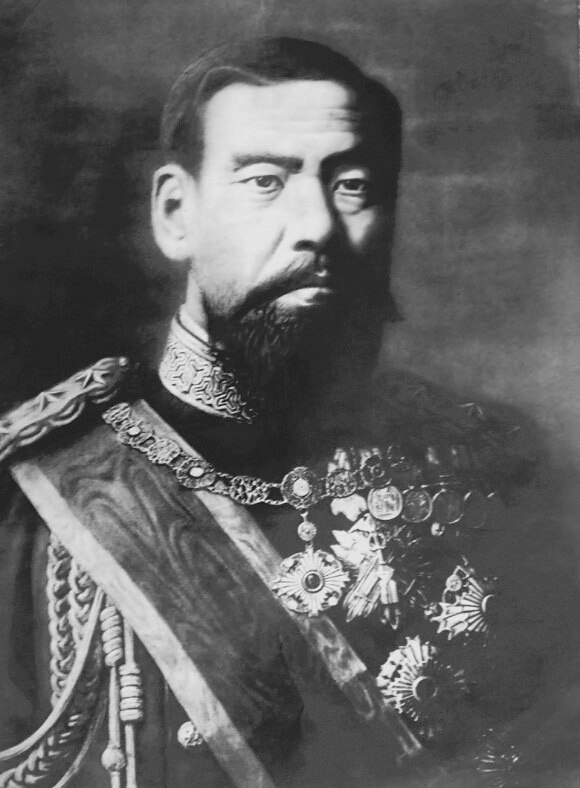
\includegraphics[scale=0.5]{Glava2/0eUExR5UGBw.jpg}
	%	\label{fig:scipion} % Unique label used for referencing the figure in-text\end{document}
	%	%\addcontentsline{toc}{figure}{Figure \ref{fig:placeholder}} % Uncomment to add the figure to the table of contents%----------------------------------------------------------------------------------------
	\caption{Император Муцухито, он же Мэйдзи}%	CHAPTER 2
\end{figure}

Можно много говорить о том, что перемены были необходимы Японии. Можно рассуждать о предпосылках стремительного рывка её от положения насильственно "открываемой" почти что уже колонизируемой, в целом слабой и мало чем, кроме любопытной национальной культуры, примечательной страны на самом краю континента, к статусу одной из великих держав. Но огромная роль императора-реформатора в том, что на этом сложнейшем пути его стране сопутствовал успех, неоспорима. Муцухито для Японии значит, как минимум, не меньше, чем Пётр Великий для России, при этом в целом воспринимается обществом куда более однозначно. Петра I я упомянул не случайно – помимо сходств, в качестве абсолютных монархов, которые решительно двинули свои государства по пути модернизации и вестернизации, между ним и Муцухито, разумеется, есть и различия.

Петр, вне всяких сомнений, сам был главным инициатором и разработчиком своих преобразований. С японским императором всё куда сложнее. Начать стоит с того, что в тот момент, когда будущий Муцухито, а тогда ещё Сатиномия (Счастливый принц), получал образование, его активное участие в государственных делах никем не предполагалось. Система сёгуната, как известно, отводила императору почти декоративную роль, а потому, главным образом, наследник Хризантемового трона изучал поэзию (позднее, уже обретя власть, он продолжит писать стихи), каллиграфию и тому подобные дисциплины. К моменту смерти его отца и восхождения на престол в 1867 году, степень осведомленности Муцухито о политических вопросах, да и вообще о положении дел в стране была очень слабой. Было ему тогда всего 15 лет. Никогда в жизни он не покидал Киото, причём, естественно, центральной его части. Но всего важнее даже не это. Сравним вновь с Петром. С ранних лет он знает, что судьба его – править. Реально, а не фиктивно. И, когда возникает препятствие в виде Софьи и её амбиций, он играет весьма активную роль в её падении, деятельно ему способствует. Значение Муцухито в деле ликвидации сёгуната и победе над Токугава Ёсинобу ничтожно. Восстание княжеств Тёсю, Тоса и Сацума началось ещё при жизни его отца, человека не старого, на которого формально и ориентировалось, а реально шло с порой на собственные силы сумевших провести частичное перевооружение по европейскому образцу армий соответствующих даймё. Решающее военное поражение сёгунат потерпел ещё в 1866. Иными словами, Муцухито не взял в свои руки власть – её ему дали. По общим оценкам вплоть до 1871 года, когда полностью было покончено со сторонниками прежней формы правления и завершилась убедительной победой новой власти так называемая война Босин, император в реальном управлении страной не участвовал. Действительно же решающим его влияние на политику сделалось только в 1880-х, когда первый этап реформ принёс по-настоящему ощутимые плоды.

К чему это всё здесь пишется? Дело в том, что начало новой истории Японии проходило при преобладании деятелей, вышедших из регионов-победителей, трёх княжеств, расположенных на юге Страны Восходящего солнца, которые и повергли династию Токугава. Причём в дальнейшем они повели себя чрезвычайно и во всех отношениях мудро. Будучи вполне готовыми сохранять власть в условиях традиционной Японии, они сознавали свою неспособность сделаться государственными деятелями новой формации, вестернизированными, по-новому образованными. Не даймё, а министрами. И озаботились воспитанием тех людей, которые должны составить их смену. Причём, хотя, конечно, заботясь о своих семьях, даймё княжества Сацума Симадзу Тадаёси, даймё княжества Тёсю Мори Такатика и даймё княжества Тоса Ямаути Тоёнори, а так же и другие ключевые лидеры, свергшие сёгунат, в качестве основного критерия ставили талант, а не происхождение. Единственным обязательным условием была принадлежность не столько к семейству, сколько к клану в самом расширительном смысле этого слова. Идеальный пример – Ито Хиробуми: 1-й, 5-й, 7-й и 10-й премьер-министр Японии, председатель Тайного совета, автор проекта первой Конституции страны. 

\begin{figure}[h!tb] 
	\centering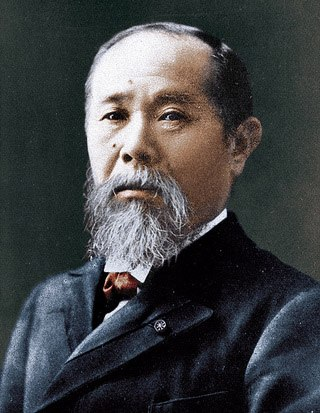
\includegraphics[scale=0.5]{Glava2/vIGO4y6PHDo.jpg}
	%	\label{fig:scipion} % Unique label used for referencing the figure in-text\end{document}
	%	%\addcontentsline{toc}{figure}{Figure \ref{fig:placeholder}} % Uncomment to add the figure to the table of contents%----------------------------------------------------------------------------------------
	\caption{Ито Хиробуми}%	CHAPTER 2
\end{figure}

Родился он 16 октября 1841 года в столице княжества Хаги, находившегося в вассальной зависимости от княжества Тёсю в крестьянской семье, однако позднее был усыновлён семейством Ито и получил статус асигару и фамилию Ито. Этого, в общем, по меркам старой, сословной Японии ничтожного статуса оказалось достаточно, чтобы показавшего большие успехи в традиционных науках мальчика включили в состав так называемой Пятёрки из Тёсю – группы юношей, для которых, впервые в истории страны и не смотря на прямой запрет тогда ещё полновластного сёгуна, в 1863 году был организован выезд на обучение Университетский колледж Лондона. Все пятеро будут в числе крупных государственных деятелей Японии периода Мэйдзи, а двое – пожалуй, ключевыми. В 1870 году, уже после победы в Войне Босин, для того же Хиробуми была организована поездка на стажировку в США для изучения валютно-финансовой системы. В 1871 он займёт видное место в крупной дипломатической миссии, посланной японским правительством в Европу.

Ну а уже в 1873 году 32-летний Ито становится министром общественных работ (строго говоря, полноценный, европейского типа кабинет министров ещё не был создан, потому иногда можно видеть и другие названия должности Ито Хиробуми, но функционал и размер полномочий, тем не менее, обозначены). Процесс перехода власти от старых элит к новым осуществлялся на редкость мягко и плавно – по любым меркам, ну а тем более по японским. Старые лидеры могли как умирать (с очень чётко составленным политическим завещанием и подготовленным преемником), или тихо отходить в сторону, что делает им честь. Конечным результатом стало образование сплочённой за счёт как землячества, так и осознания общности своей судьбы и своих политических целей, заблаговременно подготовленной прослойки крупных деятелей-реформаторов в окружении императора. Старые даймё сумели, таким образом, несмотря на решительный слом всех прежних оснований японской жизни, пересадить на новую почву часть своих наиболее принципиальных воззрений, а так же ретранслировать в будущее влияние своих родных областей, которые, получившие его ввиду того, что смогли несколько обогнать остальные регионы в деле модернизации, сами по себе, если бы не эта целенаправленно выращенная, в том числе и за границей элита, не имели бы внутренних ресурсов для его удержания.

Вопрос о том, делал ли император свиту, или свита – императора, остаётся во многом открытым в японской истории. Точных сведений о том, кто первым предлагал те или иные знаковые идеи и новации, как правило, нет. Известно, что Мэйдзи на заседаниях Государственного совета сам говорил немного – но это не обязательно означает ведомость и индифферентность. Многое решалось на неформальном уровне. И это нашло своё отражение в Конституции 1889 года, которая действовала в Японии и в 1920-х – 1930-х годах. Большие властные прерогативы императора, который, однако, практически никогда не принимал принципиальных решений, предварительно не посоветовавшись с определённым кругом людей, краткость Конституции, оставлявшей непрописанными многие вопросы взаимодействия между органами и ветвями власти. Пробелы эти порой заполнялись императорскими указами, но чаще – политической практикой. 

\begin{figure}[h!tb] 
	\centering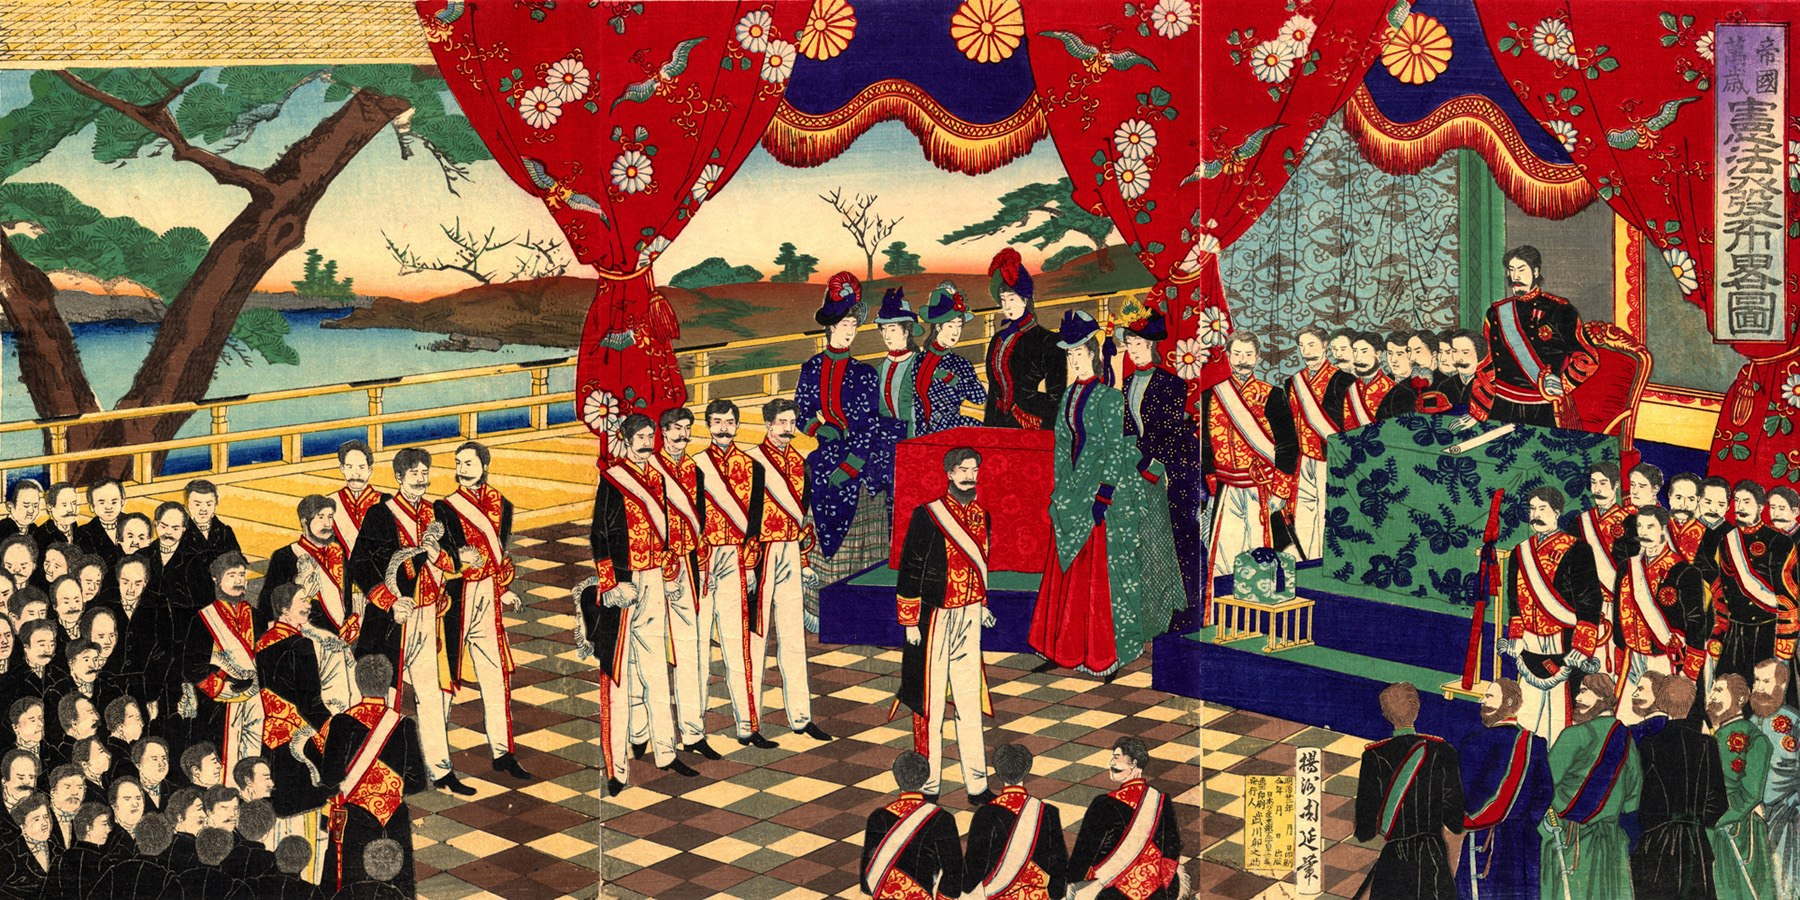
\includegraphics[scale=0.4]{Glava2/5jM5Gr9SNKY.jpg}
	%	\label{fig:scipion} % Unique label used for referencing the figure in-text\end{document}
	%	%\addcontentsline{toc}{figure}{Figure \ref{fig:placeholder}} % Uncomment to add the figure to the table of contents%----------------------------------------------------------------------------------------
	\caption{Провозглашение Конституции Японской империи в представлении представителей традиционной школы японской графики}%	CHAPTER 2
\end{figure}

\begin{figure}[h!tb] 
	\centering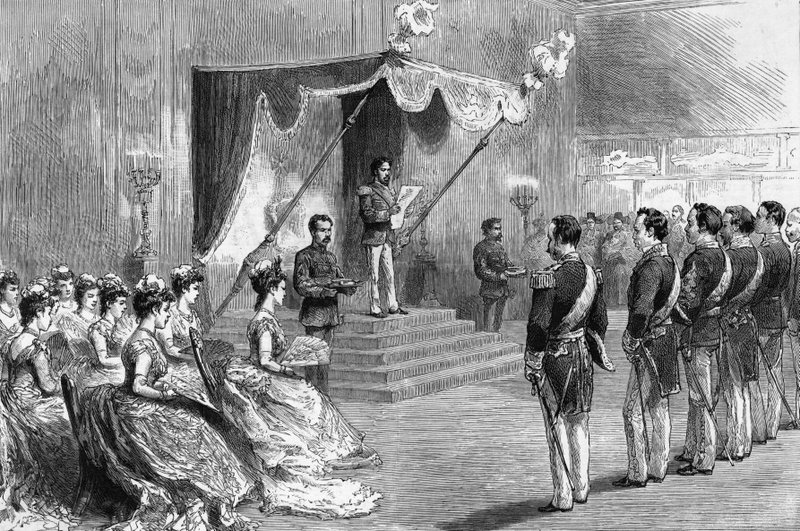
\includegraphics[scale=0.5]{Glava2/C6HfQOne0Bk.jpg}
	%	\label{fig:scipion} % Unique label used for referencing the figure in-text\end{document}
	%	%\addcontentsline{toc}{figure}{Figure \ref{fig:placeholder}} % Uncomment to add the figure to the table of contents%----------------------------------------------------------------------------------------
	\caption{Провозглашение Конституции Японской империи в представлении европейцев. Иллюстрация из журнала The Graphic}%	CHAPTER 2
\end{figure}

Формально ситуация была следующей. Основная часть конституции была прямо списана с Конституционной хартии Пруссии, в некоторых аспектах разбавленной и дополненной документами других германских государств, например Бадена и Вюртемберга. Отдельные пункты были взяты у британцев – в частности организация парламента и институт пэров. Своего было не так много. Японский учёный Накано Томио, предпринявший в 1920-х годах тщательный сравнительный анализ статей японской и европейских конституций, пришёл к выводу, что лишь три статьи Конституции Японской империи могут считаться вполне оригинальными — статья 1 о непрерывной династии, статья 31 о полномочиях императора в случае военного положения и статья 71 о применении бюджета предшествующего года.

На вершине пирамиды власти находился император. Он назначал судей, которые действовали от его имени, был главнокомандующим вооружённых сил, формировал кабинет министров, дарует статус пэра и право заседать в верхней палате парламента (который в целом имеет право по своему желанию распустить, запустив процесс перевыборов). Подданные могли выбирать только нижнюю палату парламента – Палату депутатов. 

\begin{figure}[h!tb] 
	\centering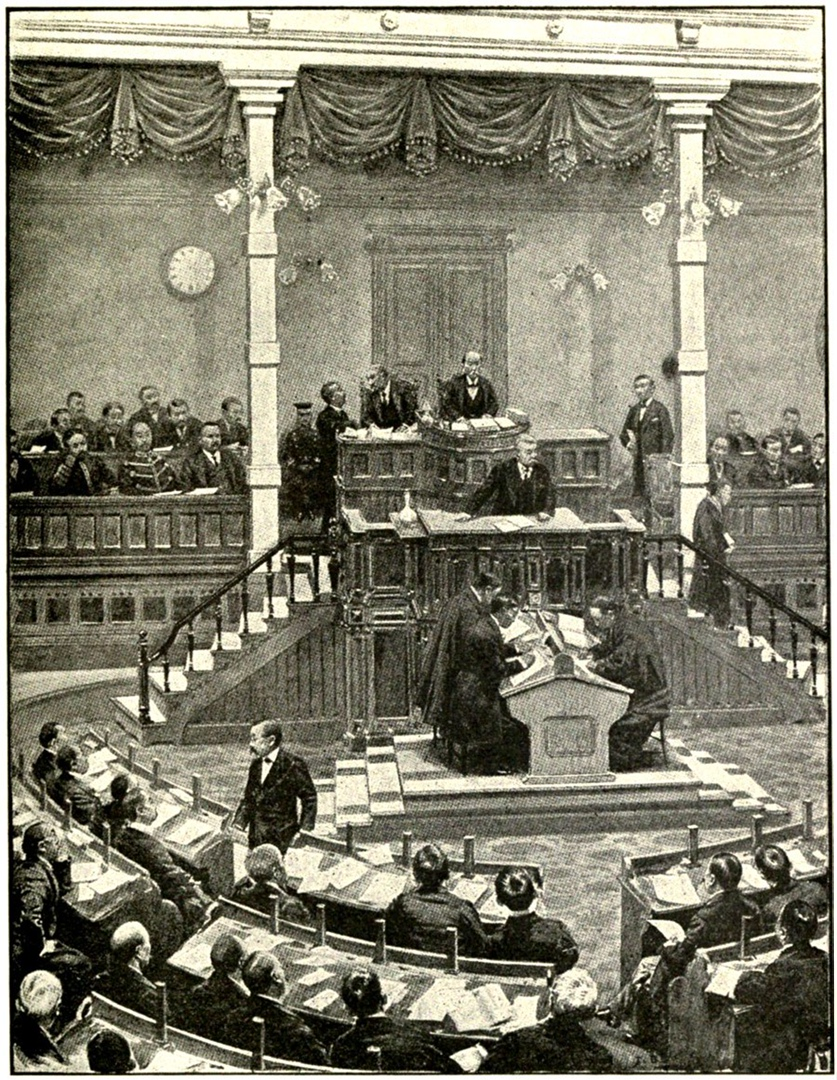
\includegraphics[scale=0.5]{Glava2/z8Rrmsg8n38.jpg}
	%	\label{fig:scipion} % Unique label used for referencing the figure in-text\end{document}
	%	%\addcontentsline{toc}{figure}{Figure \ref{fig:placeholder}} % Uncomment to add the figure to the table of contents%----------------------------------------------------------------------------------------
	\caption{А вот так на самом деле выглядел японский парламент}%	CHAPTER 2
\end{figure}

Однако, перечисление органов власти на этом не окончено. Существовал ещё Тайный совет, члены которого также назначались императором. Теоретически единственная функция Совета – сугубо совещательная, т.е., собственно, давать Микадо те или иные рекомендации – не более. Фактически же, ситуация напоминала ту, которую мы можем видеть в современной России в отношениях между правительством, парламентом и администрацией президента. Но и это ещё не всё, потому, что существовали Гэнро.

Это – совершенно особенное явление японской политической жизни и культуры. По большому счёту, весь предшествующий текст этой главы был написан для того, чтобы подвести к ним и их роли. В отличие даже от Тайного совета, Гэнро – это вообще не орган государственного управления. Гэнро – не должность и не чин. Это статус. Гэнро – всего их было 9 (но не одновременно, а в течение всего периода правления Муцухито), это ключевые деятели эпохи реформ, основные сподвижники императора Мэйдзи в деле перелицовывания страны. Только в Японии, вероятно, возможна такая тонкая грань формального и неформального, как в этом случае. Существовала особая церемония "производства" в гэнро – но не все из девятки её прошли, что никак и ни на что не влияло. С гэнро почти как с дао – проще перечислить чем оно не является, чем дать точное определение. Это не орден, не тайное общество, не титул. Фактически, как бы странно это не прозвучало, это такой особый вид императорской признательности – и императорского же личного обязательства перед этими людьми. Ни в каком документе, тем более в Конституции, полномочия совета Гэнро не прописаны. Реально император почти ничего не делал без их принципиального одобрения. Именно гэнро предлагали (но не всегда, а только тогда, когда сами считали нужным) императору кандидатуру на должность премьер-министра, и император во всех случаях принимал их рекомендацию. Мэйдзи добровольно разделял с ними свою власть, что давало возможность девятке менять уже формальные свои статусы как рабочую одежду. Министры, генералы, наместники, они могли потом на время уходить в тень – и вновь возвращаться на свет с новым указом монарха. Власть гэнро, никак и нигде иначе не закреплённая, осуществлялась через прерогативы и полномочия императора, который, таким образом, очень мудро гарантировал её сохранение и поддержку самыми видными и талантливыми государственными мужами страны, которые в ином случае могли бы по тем или иным соображениям пытаться ограничить, а то и подточить её. Гэнро были нужны императору, но и он был необходим гэнро.

Современная историография Страны Восходящего солнца называет их отцами-основателями Японии, проводя параллель с американскими. Определённое рациональное зерно в этом есть. Люди это и вправду были выдающимися – и роль в трансформации своего отечества в могучую силу сыграли большую. Формат гэнро был удобен, судя по всему, лично Мэйдзи, соответствуя его характеру, достаточно выгоден для не имеющей опыта парламентской демократии страны, близок к меритократии, как её описывал, например Платон – власти мудрых и не ограниченных условностями. Но…

Система эта с гарантией программировала в будущем глубокий политический кризис. Вожди борьбы с сёгуном могли заранее подготовить себе преемников потому, что власть в стране была ещё совершенно не институционализирована. Не было не то что Конституции, представительства, но почти вообще ничего. Избранные ими люди, пройдя через горнило реформ, обретя опыт, сработавшись с императором, сделались гэнро. Они же выстроили по кирпичу здание новой государственности, продолжая негласно направлять общее движение страны в море большой политики. Но и они, и сам император – смертны. И невозможно передать, ни по наследству, ни в виде чинопроизводства пост "сподвижник великого императора". Вернее, при большом таланте к политическому эквилибру, возможно всё, но в Японии конца XIX – начала XX века до такого ещё не дошли. А теперь вернёмся к тому, с чего начали – в 1912 умер Мэйдзи. Ещё в 1909 – Ито Хиробуми, первый и наиболее влиятельный из гэнро. До него в 1900 умер Курода Киётака, а в 1902 - Сайго Цугумити. В 1913 умрёт Кацуро Тара, в 1915 – Иноуэ Каору… К концу Первой Мировой в живых останется три гэнро. К моменту принятия решения об интервенции в Манчжурию в 1931 – один.

При этом ни один из легальных и публичных органов и институтов власти не был достаточно силён, чтобы взять в свои руки бразды правления. Народовластие было, помимо прочего, ограничено жесточайшим избирательным цензом, основанном на величине доходов. При том, что на первых выборах в Палату депутатов в 1890 году проголосовало 94\% тех, кто имел на это право, это был менее чем 1\% населения страны. Кабинет министров находился в никаким законом не обусловленной, но жесткой зависимости от Тайного совета, а тот в свою очередь прежде направлялся гэнро, а теперь – непонятно кем. Вообще во все предшествующие годы – причём от момента их создания - иных прецедентов они не знали, все эти органы не только были на практике, но делались намеренно и целенаправленно ограниченно самостоятельными. Гэнро не только увязывали их на себя, но и служили совершенно необходимым механизмом координации, объединения и направления усилий.

Из предыдущей части должно было стать ясно, почему в Японии, несмотря на наличие мощных финансово-промышленных объединений, не сформировалась классическая олигархия. Самоуправление отсутствовало как класс. Местные элиты были целенаправленно подавлены сперва территориальной реформой Мэйдзи, которая уничтожила исторические провинции страны, переделив их между новыми префектурами, а после и рядом других мер, в том числе карательного характера. Вот и получалось, что власть не то чтобы лежала на земле, как это было, скажем, у нас в 1917, но не было никого, кто обладал бы ею в полной мере. Теоретически Конституция давала исключительные, почти самодержавные возможности в руки императора – но в объективной реальности Японии 1910-х он уже не мог быть самодержцем – вместо могущества и полновластия он, напротив, повис бы тогда в воздухе, а после, несмотря на огромный пиетет к правящему дому, оттеснён на прежнее, декоративное место, которое занимал до Реставрации Мэйдзи. Быть может кто-то со стальной волей и могучим интеллектом и мог бы реально использовать свои прерогативы и права, но те люди, которые на самом деле последовали за Муцухито (а уже он, как мы поняли, руководил страной отнюдь не самовластно), были на это совершенно не способны.

У Мэйдзи было 15 детей, однако до зрелых лет дожило лишь пять, из которых 4 были девочками, а японская традиция, в отличие даже от Китая, не знает правящих императриц. Таким образом, хотя до 1889 года не существовало документа, который определял бы порядок престолонаследования, т.е. теоретически права действующего императора в этом вопросе ограничены не были, но в действительности альтернатива принцу Хару (позднее получившему имя Ёсихито) отсутствовала. 3 ноября 1889 года он был официально провозглашён наследником. 
\begin{figure}[h!tb] 
	\centering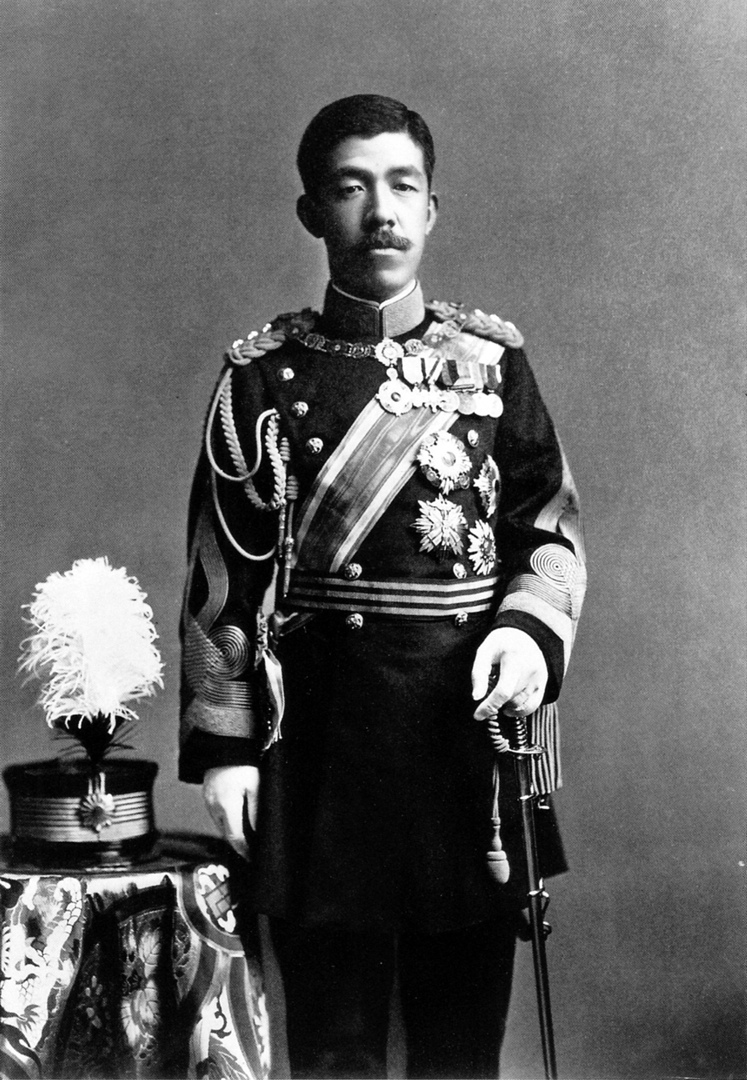
\includegraphics[scale=0.5]{Glava2/UPgOys64H08.jpg}
	%	\label{fig:scipion} % Unique label used for referencing the figure in-text\end{document}
	%	%\addcontentsline{toc}{figure}{Figure \ref{fig:placeholder}} % Uncomment to add the figure to the table of contents%----------------------------------------------------------------------------------------
	\caption{Ёсихито, уже в ранге императора Тайсё}%	CHAPTER 2
\end{figure}

Сложно сказать, что представляло бы собой правление императора Ёсихито. Никакими особыми способностями он не блистал и никак не проявил себя в детские годы – впрочем, его великий отец тоже стал таковым не сразу. Но всё это – лишь догадки. Дело в том, что будущий император с девизом правления Тайсё (великая справедливость) в детстве переболел менингитом, что сказалось на нём самым фатальным образом. Это касалось и физического и, в первую очередь, умственного здоровья. Наследника, а затем и монарха то охватывали приступы почти беспричинного гнева, во время которых он доходил до того, что бил окружающих своим жокейским хлыстом, то на их место приходили волны ужаса. Ёсихито страшно боялся покушения на свою жизнь. Состояние его было хорошо известно, так что нет ничего удивительного в том, что под предлогом траура по Муцухито, церемонию интронизации и передачу власти наследнику отложили аж на три года – до ноября 1915. Помимо простого и понятного желания подольше не иметь дела с полубезумным человеком на троне, был и ещё один мотив – все, и не без оснований, боялись, что Тайсё может провалить церемонию и страшно опозориться сразу в начале царствования. Уже позже, сделавшись императором, во время одного из парадов Ёсихито совершенно неожиданно и без видимых причин упал с лошади и не мог сам подняться.

По большому счёту, единственное, что император был просто обязан сделать – и, по возможности, качественно – это сына-наследника. С 10 мая 1900 Тайсё был женат на принцессе Садако. Именно Ёсихито ввёл при дворе моногамию – до того, помимо главной, официальной жены, император имел множество наложниц. Есть, впрочем, предположение, что дело тут было не в каких-то новых, по сравнению с предшественниками, моральных принципах и воззрениях, а банально в том, что немощному императору одной женщины было более чем достаточно. Как бы там ни было, Тайсё и Садако со своими обязанностями справились успешно – один за другим на свет появились четыре принца, причём все достаточно здоровые, успешно пережившие годы младенчества и детства. Старшим был рождённый 29 апреля 1901 года принц Мити, который получил титул наследного принца 2 ноября 1916. 

\begin{figure}[h!tb] 
	\centering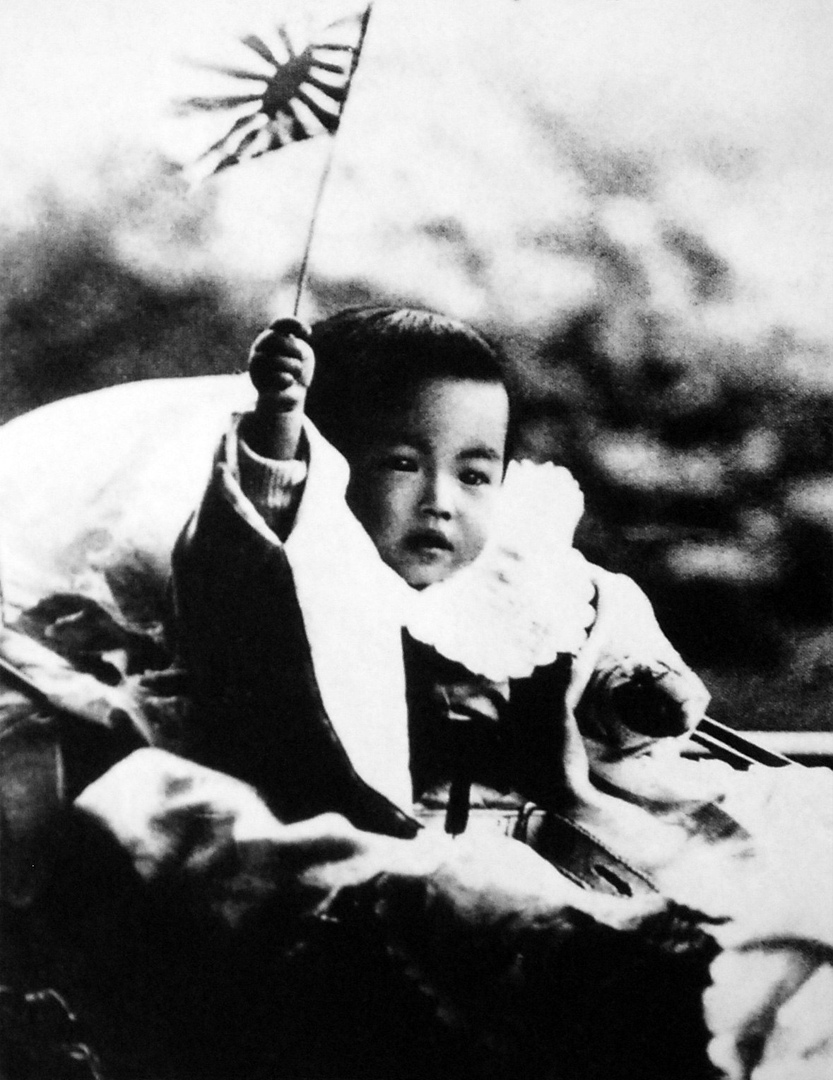
\includegraphics[scale=0.5]{Glava2/twkoleSHWaI.jpg}
	%	\label{fig:scipion} % Unique label used for referencing the figure in-text\end{document}
	%	%\addcontentsline{toc}{figure}{Figure \ref{fig:placeholder}} % Uncomment to add the figure to the table of contents%----------------------------------------------------------------------------------------
	\caption{Принц Мити, будущий Хирохито, в возрасте 2 лет}%	CHAPTER 2
\end{figure}

На мальчика многие смотрели с надеждой – состояние его отца с годами лишь ухудшалось. Во время своего последнего появления в парламенте в 1919 году он, вместо того, чтобы произнести заранее подготовленное слово, молча свернул в рулон текст своей речи и, держа ее как подзорную трубу, таращился совой на поднимающихся с места и кланяющихся парламентариев. Хотя, конечно же, никаких проявлений непочтительности не было, с этого момента правление Тайсё фактически подошло к концу. Большую часть времени император начинает проводить на загородных виллах вне Токио под заботливым, но плотным присмотром. А уже в 1921 году при императоре был официально назначен регент – его успевший как раз подрасти 20-летний сын Хирохито. Т.е. даже строго формально Тайсё правил менее 6 лет. На самом же деле – в полном смысле слова не правил никогда. В 1926 году Ёсихито умрёт в возрасте 47 лет. Совершенно очевидно, что при Тайсё не могло возникнуть не то что новых гэнро – он вообще не оказал практически никакого влияния на состояние и состав политической элиты. Есть, конечно, как это часто бывает, конспирологические версии, согласно которым доброго и умного императора не то травили, не то обманывали много лет, а потом сжили со свету коварные и не желавшие реформ приближённые, ну да оставим их на совести тех, кто их выдумывает…

Если вернуться, держа в памяти судьбу несчастного Ёсихито, немного назад, то риски, грозившие Стране Восходящего солнца, начинают выглядеть куда рельефнее. Объективно уход поколения гэнро и смерть (надо добавить, в ещё отнюдь не старом возрасте) императора-реформатора Мэйдзи, оставляла для Японии три альтернативы. Первая – идеальная, но едва ли возможная – появление на троне не менее сильной, но, в то же время, способной к компромиссам, ценящей добрую помощь и склонной к делегированию части своей власти личности, эдакого Мэйдзи 2.0, вокруг которого естественным образом сформируется своя команда – новые гэнро. Как мы уже поняли, произошло прямо противоположное. Вторая – полное крушение здания власти, вплоть до революции – к слову, хотя у нас мало кто об этом знает, но несколько раз в своей истории Япония была на грани именно такого развития событий. В дальнейшем об этом будет сказано подробнее. И третья – некий институт, может быть даже и не имеющий на то законного права, все же получит мандат доверия от элит и общества, своеобразный ярлык на власть, а сам – не побоится принять его.

Именно это и случилось, а институтом таким сделалась армия. Почему именно она? Тому много причин. Первая – это её репутация. Если для Страны Восходящего солнца в целом эпоха Мэйдзи – это совершенно потрясающий прорыв и успех, то слава армии, конечно, особенно для японского обывателя, сияла так ярко, как ничто другое. Перемены во внутренней жизни нередко были и болезненными. О “старых-добрых” временах особенно сильно не вздыхали, но какие-то претензии к реформаторам (естественно, не к самому императору) были у многих. Армия же одерживала всем очевидные, понятные, приятные и вызывающие гордость победы, причём одну за другой. Японо-китайская, Русско-японская, Первая мировая – у всех в Японии было ощущение, что этот и без того впечатляющий список может быть и будет продолжен. Вторая причина – в том, что армия, как казалось многим, причём уже не только неискушённым в политике простолюдинам, это та сила, которая стоит вне внутренних дрязг партий и элитных групп, а защищает государство как таковое и в целом. Переползание власти в руки военных началось в значительной мере с того, что у политиков возникла примерно такого плана мысль: “Пока мы не разберёмся с нашими внутренними проблемами, не спланируем и не подготовим новую систему распределения полномочий и ответственности, нужно, чтобы кто-то надежно и без лишних вопросов и амбиций охранял то, что уже существует, подпирал старое здание, пока мы не решили, как именно его перестраивать”. И действительно, поначалу армия играла роль чисто консервативной силы, сдерживавшей напор разного рода радикалов, в то время как гражданское руководство искало пути для дальнейшего движения вперёд.

Какие именно пути? Скажем, во второй половине 1920-х, была предпринята попытка подменить гэнро так называемыми дзюсинами – бывшими премьер-министрами, которая, естественно, потерпела полный провал. Во-первых, их было слишком много. За период с 1918 по 1940 успело смениться 20 (!) премьеров. Во-вторых, сам по себе факт пребывания в этой должности и близко не соответствовал авторитету сподвижника Мэйдзи. Если гэнро, люди весьма разные, тем не менее, составляли общую “корпорацию”, то дзюсины во-первых нередко относились друг к другу весьма прохладно (и не удивительно – некогда один из них вполне мог подсиживать и интриговать против другого), а главное – не составляли никакого единства. Каждый из бывших премьеров был силён и авторитетен ровно настолько, насколько сам своей предшествующей политической карьерой смог этого добиться. Кто-то, как, скажем, принц Коноэ, был весьма влиятелен, а кто-то - совершенно нет. Не было и того особого взаимодействия между дзюсинами и императором, которое имело место между Мейдзи и его гэнро. С Тайсё вообще нельзя было политически взаимодействовать, а Хирохито не имел ни особенных поводов, ни желания устанавливать такие отношения с бывшими премьерами. В итоге получился просто клуб советников – без ответственности, но и без прав, которые, к тому же, зачастую советовали очень разное.

Были и другие попытки. Так, ещё в 1892 году, при Мэйдзи, один из гэнро – явно с ведома остальных и самого императора, попытался организовать политическую партию, носившую название Народная лига, но создать массового проправительственного движения толком не получилось. 

\begin{figure}[h!tb] 
	\centering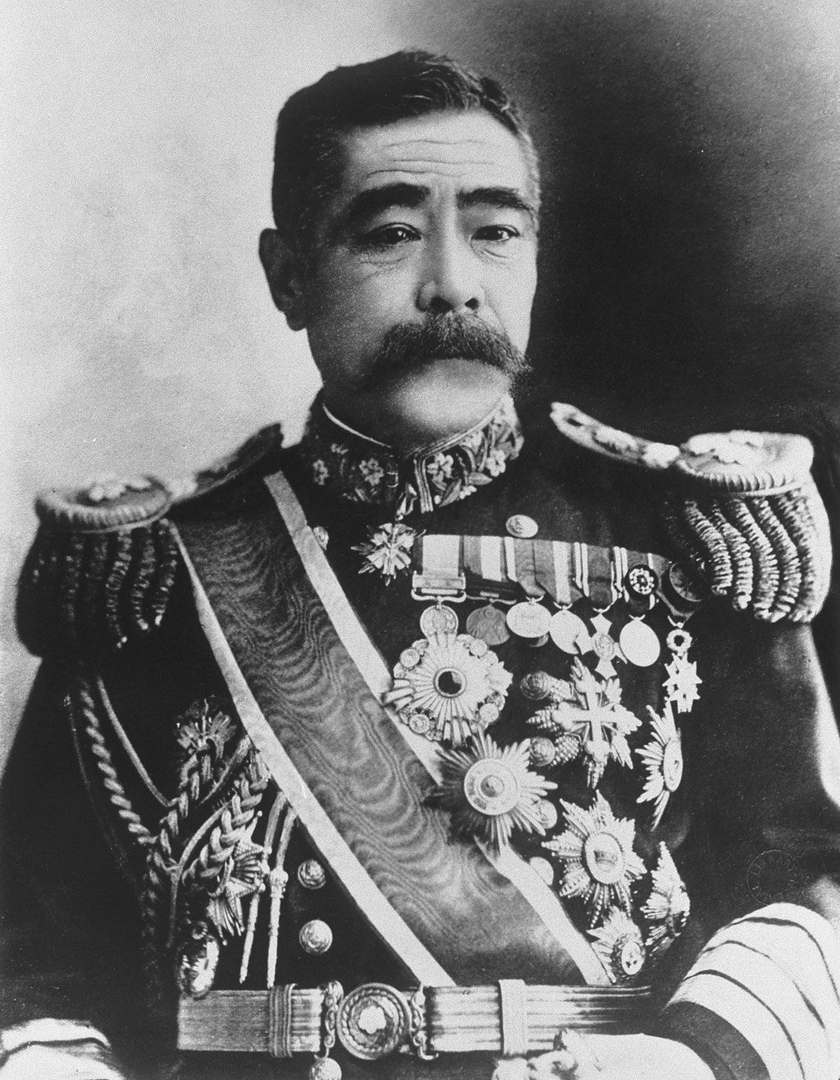
\includegraphics[scale=0.5]{Glava2/oX2fBPYepVY.jpg}
	%	\label{fig:scipion} % Unique label used for referencing the figure in-text\end{document}
	%	%\addcontentsline{toc}{figure}{Figure \ref{fig:placeholder}} % Uncomment to add the figure to the table of contents%----------------------------------------------------------------------------------------
	\caption{Сайго Цугумити, один из гэнро, маршал флота Японской империи, основатель Народной лиги}%	CHAPTER 2
\end{figure}

Японцы в массе своей были, безусловно, лояльны правящей династии и удовлетворены теми людьми, которые группировались у трона, но, именно по этому, предпочитали заниматься своими, неполитическими делами. В итоге, когда последовательно началось усиление сперва коммунистов, а потом националистов, правительству оказалось некого им противопоставить, кроме полиции и других силовиков. Тем более не удалось запустить и подконтрольный власти механизм социального лифта. Едва не единственным таким лифтом, к слову, была, как раз, армия и флот, где самурайское происхождение ценилось (впрочем, это могли быть самые бедные и неродовитые семьи), но не было жестким блоком, стеклянным потолком, который не давал бы талантливому и упорному человеку пробиться выше.

Ну а третьей причиной было то, что у армии, единственной из всех, был ясный и ей самой, и остальным план того, что нужно сделать для обеспечения благополучия и процветания Японии. Давить на Китай! Такой подход был удобен многим и во многих отношениях. Про осознанную необходимость экспансии подробно было сказано в предыдущей части. Дополнительно те же дзайбацу интересовали всё возрастающие военные заказы. Элиты были рады возможности сплотить нацию перед лицом внешних вызовов. Консерваторы радовались тому, что этот путь не требует радикальных реформ внутри страны. Дезорганизованная уходом поколения Мэйдзи-гэнро бюрократия империи получила понятную задачу, которая, к тому же, дополнительно укрепляла и усиливала её – поддерживать нацию в состоянии готовности к войне. И вот вам корни того самого пресловутого “японского милитаризма” о котором мы можем прочитать, скажем, в наших школьных учебниках.

Но был, помимо перечисленных выше причин, совершенно конкретный спусковой крючок, который очень сильно поспособствовал росту значимости армии. Как уже было сказано в самом начале этой части, помимо смерти Мэйдзи – события внутрияпонского, было и ещё одно, оказавшее огромное влияние на будущее Страны Восходящего солнца. 12 февраля 1912 года в Китае завершилась Синьхайская революция, император Пу И (мы ещё вспомним о нём позже) отрёкся от престола, Манчжурская династия пала, а Поднебесная была провозглашена республикой. Всё это обещало великие перемены, которые могли оказаться как очень выгодными для Японии, так и очень опасными. Для того, чтобы понять почему, нужно кратко остановиться на предшествующей истории Китая вообще и его отношений с японцами в особенности.

В целом, Поднебесная, меняя династии, названия, до некоторой степени – границы, тем не менее, многие века оставалась безусловным гегемоном Восточной Азии. Причём не только в военно-политическом смысле, но и в экономике, науке, культуре. Японцы никогда не признаются в этом до конца – в первую очередь самим себе, но степень заимствованного из Китая в их истории и традициях очень велик. Буддизм, конфуцианская этика, да что уж там – даже чайная церемония пришли с континента. В то же время, Япония никогда не была не только частью империи, но даже её вассалом, в отличие, например, от будущего Вьетнама, или, что важнее, Кореи. В своё время объединивший Японию после периода междоусобиц Тоётоми Хидэёси направил в силу целого комплекса причин, где, пожалуй, основной было стремление найти занятие для в одночасье ставших ненужными с установлением внутреннего мира многочисленных воинов профессионалов, свой удар на Страну Утренней свежести в 1592 году. Лёгкость побед закалённых и хорошо вооружённых японцев, а также известная внезапность их ударов привела к быстрому и полному успеху в Корее, за которым последовало самое настоящее головокружение. Сёгун возмечтал ни много ни мало завоевать Китай. Чего здесь было больше – спеси, неинформированности, или отрыва от реальности в окружении льстецов, сказать трудно. Но фактически речь шла о реализации басни про бодание телёнка с дубом в масштабах довольно многочисленной и сильной нации. Боевые действия длились 6 лет и носили довольно парадоксальный характер: японцы куда чаще побеждали своих противников, нежели им проигрывали, но стратегически Страна Восходящего солнца всё более и более истощалась, в то время как китайцы, хотя и часто терпя поражения, были способны вести такую войну ещё многие годы без особенного напряжения. Ну и, конечно, не было и речи о японском вторжении на территорию собственно Поднебесной – все события происходили в Корее. В итоге, как только упрямый, но в остальном неглупый и твёрдо державший власть в своих руках Тоётоми Хидэёси умер, обе стороны, формально не заключив мира, сочли за благо свести войну на нет. Ну а позднее, после долгих и порой курьёзных переговоров, дипломаты двух стран всё же сумели это официально закрепить и оформить.

Эта история, отстоящая от рассматриваемого нами периода более чем на три столетия, тем не менее, очень поучительна и мы будем вспоминать её, когда поведём речь о начале открытой войны Японии с Китаем уже в 1930-е годы. А тогда, на рубеже XVI и XVII веков, Китай был для японцев явно не по зубам – так оно было и в дальнейшем. Как следствие, никаких военных поползновений в период сёгуната Токугава, что на Поднебесную, что даже на Корею, не предпринималось. Вообще для всех в Азии, а с войны 1592-1598 годов и для японцев, величие Китая было как бы константой, которую никто не ставил под сомнение. Ну, почти никто – кочевники были всегда самой страшной головной болью для великой империи. И в 1644-1683 они, а именно манчжуры, завоевали Китай в последний раз. Довольно быстро, как и всегда, Китай оправился, частично переварил и ассимилировал своих покорителей, вернул свой статус и возобновил традицию (скажем, экзаменов на соискание чиновного поста). Весь XVIII век империя Цин только разрасталась и крепла. В новое, XIX столетие, она входила самым населённым государством мира с крупнейшей армией и неизменно положительным торговым балансом, в том числе со странами Европы. Однако уже скоро наступит период величайшего в истории Поднебесной унижения – Опиумные войны. Пересказывать их причины и ход здесь нет ни места, ни нужды, ограничимся обобщённым итогом – горстка европейцев сокрушила непобедимую империю, продиктовала ей свои условия, создала торговые фактории и базы, в частности знаменитый Гонконг, которые позволяли дополнительно контролировать соблюдение достигнутых договорённостей. Китай был насильственно “открыт” – и его экономика, а скоро после неё – и государственный аппарат, начали рушиться, оползать и рассыпаться, так что не удивителен тот внутриполитический эффект, который оказало на японцев прибытие эскадры коммодора Перри – слишком показателен и печален был пример соседей. Ответом на вызовы времени стала ускоренная модернизация. Казалось бы, Китай должен был пойти этим же путём. Однако, не вышло.

Причин тут много. Но, пожалуй, ключевая, это оторванность он основной части народа Манчжурской династии и элиты в целом, причём не только политическая, социальная, экономическая, но и этническая. Нельзя, конечно, говорить, что Китай больше двух с половиной столетий находился в оккупации, как это делали в своё время ультрапатриоты, но факт остаётся фактом – фактор крови, пусть уже во многом иллюзорный, продолжал играть свою роль в распределении властных полномочий. Императоры, уже совершеннейшие китайцы, и по культуре, и по этносу (тут постаралась масса наложниц), тем не менее, продолжали поддерживать старые и отжившие перегородки в обществе, боясь, что без них их власть рухнет.

В Японии Мэйдзи был возведён на трон как действительный властитель теми, кто хотел перемен, сам возглавил этот процесс, доверяя в то же время своему окружению. Японцы в целом, видя последовательность и решимость власти, не стеснялись учиться и не боялись меняться. В Китае императоры балансировали между группировками реформаторов и консерваторов, попеременно поддерживая то одних, то других, с единственной целью обезопасить и подкрепить собственную династию. Даже когда реформаторы преобладали, их победа никогда не была полной. Китайцы могли покупать технику, особенно оружие, но в полном смысле переучиваться не желали и не могли. Шли бесконечные дискуссии о том, что можно и что нельзя брать у Запада, в какой момент принятие иностранных образцов затронет суть и соль жизни Поднебесной, можно ли это допустить и всё в таком духе. Обязательная система экзаменов, некогда гордость Китая, теперь привела к тому, что воспроизводились исключительно консервативные и не готовые к ломке старого деятели. Отдельных смельчаков и самородков давили массой.

Наконец, по мере углубления кризиса, множились восстания, причём, к сожалению, они были очень далеки от прогрессивных революций – в основном это были дикие бунты тех или иных специфических для Китая помесей тайных обществ и сект. Ярчайший пример – восстание тайпинов. Занятно, что сами себя тайпины полагали христианами, хотя, если бы их воззрения удалось в полной мере донести до католического, протестантского, или православного священника той эпохи, то у любого из них волосы бы встали дыбом. 14 лет с 1850 по 1864 год они пожирали огромные ресурсы государства, направляемые на борьбу с ними. Что ещё хуже, в конечном счете, правительство Китая было вынуждено нанять европейских военных специалистов на командные должности в армии, чтобы справиться с ними. Самый известный пример – британский генерал Гордон, чья слава родилась именно тогда. Почему приглашение военспецов было опасно? Да потому, что у них толком не учились, затвердив и переняв только отдельные внешние формы, зато на будущее многие политические и военные лидеры Китая были убеждены, что уже видели и постигли эту самую загадочную европейскую военную науку.

К концу XIX века Китай пришёл в ужасающем состоянии, чем и воспользовались японцы. Война 1894-1895 года очень сильно ударила по застоявшимся умам. Можно было примириться с поражениями от белых. Но то, что японцы – здешние, такие же, да что там, всегда худшие, более слабые по сравнению с великой и могучей Поднебесной империей, победили Китай...! После такого унижения страну начало трясти не по-детски. Боксёрское восстание – классический пример того, как властьпридержащие пытаются канализировать под своим контролем скопившийся протестный потенциал, возглавить народное движение, выпускают джинна из бутылки, а потом страшно его пугаются, но уже не могут загнать обратно. Императрица Цыси сперва явно потворствовала ихэтуаням, а потом была бессильна от них избавиться и полностью утратила над ними контроль. Но были и другие силы. Нападения на посольства оказались как нельзя лучшим поводом. Возмутились все ведущие страны цивилизованного мира, а их правительства поспешили этим законным негодованием на действия агрессивных дикарей, воевавших в числе прочего с телеграфными столбами, воспользоваться. Альянс восьми держав – вещь в истории беспрецедентная. Ни до, ни после никогда не было такого случая, чтобы объединились в едином строю без изъятия все основные мировые державы. Сочеталось, как кажется, несочетаемое, например немцы и французы. В Альянсе были представлены: Германия, Франция, Россия, Япония, США, Британия, Италия и даже не имеющая колоний и почти сугубо сухопутная Австро-Венгрия. В некотором роде это был тогдашний аналог миротворческого контингента ООН. 45 000 солдат под командованием немецкого генерал-фельдмаршала Вальдерзее достаточно быстро справились с противником. Весь вопрос был – что потом?

Китай стремительно превращался в некий аналог Османской империи, в больного человека Азии, слабого, почти агонизирующего, но слишком большого, чтобы какая-нибудь одна колониальная держава могла заглотить его разом. Иными словами, Поднебесную не делили в первую очередь потому, что опасались в процессе позволить получить слишком жирный кусок и слишком большие преимущества своим противникам и конкурентам. Эта система сдержек, как кажется, работала, но прочной ей назвать было никак нельзя. А главное – время движется вперёд. Та же Высокая порта на глазах в том числе и японцев начнёт лавинообразно терять территорию после прихода к власти младотурок. Италия отберёт Ливию, 1-я Балканская война едва не сократит европейские владения турок до одних только окрестностей Стамбула. Когда в 1911-1912 грянуло в Поднебесной, у японцев было обоснованное (и частично подтвердившееся) подозрение, что ситуация может начать развиваться по аналогичному сценарию. Иначе говоря, державы, сочтя новое правительство слишком нестабильным для поддержки, могут бросить свои заботы над больным человеком, и позволить событиям идти естественным путём. В этом случае для Японии было критически важно оказаться в числе первых в очереди за наследством.

Однако, мы несколько забежали вперёд. Прямым следствием Восстания боксёров стало ускорение действий русского правительства в Манчжурии и в целом расширение его амбиций. Китай был слаб, так что теперь туда лезли буквально все, как в вокзальный буфет. После японско-китайской войны Российская империя выступила в качестве друга, почти союзника китайцев. Теперь, после достройки КВЖД, проведении необходимых работ (первого их этапа) в Порт-Артуре и Дальнем, с ними стали считаться в гораздо меньшей степени. Если вместе с китайским правительством Россия действовала по необходимости умеренно, ибо власти Поднебесной просто не могли совершать излишне резких движений, то теперь дела пошли много более напористо. Ключевым же было то, что Восстание дало возможность наплевать на ранее заключенные договорённости о выводе русских войск с территории Китая.

Мы не станем здесь подробно останавливаться на причинах и ходе Русско-японской войны – это тема для полноценной отдельной работы, а то и целого ряда работ. Не станем мы акцентировать внимания и на причинах нашего неуспеха и японской удачи. Ключевое для нас – это то политическое и моральное влияния, тот эффект, который вызвал успех Империи Восходящего солнца в Азии. В том числе и в Китае. С одной стороны, война ещё раз и очень унизительным образом продемонстрировала его слабость – она, хотя об этом часто забывают, шла, собственно, на китайской территории, при том, что официальное правительство в Пекине сохраняло нейтралитет, не давало никому и никаких разрешений на подобные действия, а, за исключением сданного в аренду Ляодунского полуострова, именно оно было законным правительством в Манчжурии. Фактически ситуация была следующей: третьи страны вели масштабные боевые действия на территории Китая, не спрашивая и вообще не замечая его – и он ничего с этим не мог поделать. Куда уж позорнее! С другой, произошло немыслимое – азиатская страна выиграла у европейской. Перворазрядной великой державы! Полновесную, масштабную войну! Без союзников! Вообще в мире победа Японии была сенсацией, но в Азии это было событие, переворачивающее мир.

Ничто иное не могло дать такого импульса и толчка, так усилить сторонников реформ и перемен, как этот потрясающий пример! Всякие сомнения теперь развеивались, а контраргументы парировались такими словами, как Порт-Артур, Мукден и Цусима. Азиатское государство добилось в мирном договоре с европейским территориальных уступок (пусть Полусахалинский граф Витте и сделал всё, чтобы они были минимальными и совершенно ничего не значили для империи, кроме некоторой потери престижа). Да, в реальности у японцев всё было не так радужно, как могло показаться неискушённому наблюдателю. Несмотря на свои неоспоримые победы, страна была сильно истощена, а Россия, пожалуй, могла бы даже рассчитывать на итоговый успех, в случае концентрации всех своих усилий на Дальнем Востоке. Вот только именно этого по причинам дипломатическим и военно-стратегическим, экономическим, социально-политическим и прочим она и не могла сделать. Очень велики делались риски.

Новые народные восстания в Китае были неминуемы, но они вполне могли быть повторением того, что имело место в случае с тайпинами, или боксёрами – слабоорганизованное движение, основанное не утопических представлениях и принципах. Теперь же в Китае появилась прослойка интеллектуалов и даже чиновничества, которая знала что именно нужно стране, а образцом в значительной мере видела именно Японию. Основатель Гоминьдана, один из отцов Синьхайской революции, человек, которого почти в равной мере почитают в современных КНР и на Тайване, Сунь Ятсен сделал решающий шаг по пути борьбы именно в 1905 году – и это не случайно. Не менее знаковым можно счесть и тот факт, что в этот момент, когда он основывал свой революционный союз борьбы Тунмэнхой, Сунь Ятсен находился не где-нибудь, а в Токио. 

\begin{figure}[h!tb] 
	\centering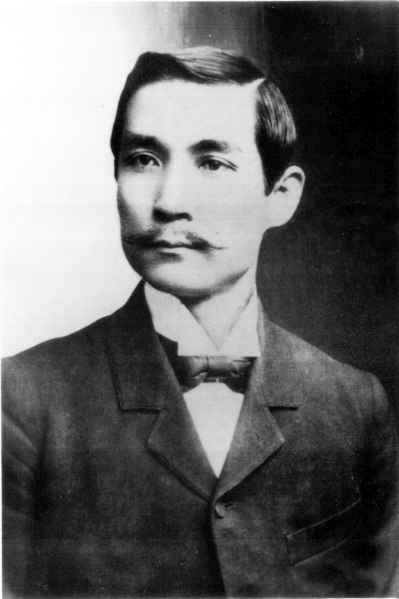
\includegraphics[scale=0.5]{Glava2/UtLNSsPuDcE.jpg}
	%	\label{fig:scipion} % Unique label used for referencing the figure in-text\end{document}
	%	%\addcontentsline{toc}{figure}{Figure \ref{fig:placeholder}} % Uncomment to add the figure to the table of contents%----------------------------------------------------------------------------------------
	\caption{Примерно так Сунь Ятсен выглядел в те годы}%	CHAPTER 2
\end{figure}

Отношение китайцев к Стране Восходящего солнца в это время было очень двойственным: с одной стороны, её боялись, а так же не могли не припоминать ей поражений и унижений недавней войны. С другой – у неё жадно учились и истово на неё надеялись, как на пример того, что азиатская страна может достигнуть успеха, двигаясь по пути модернизации. Едва ли не большинство лидеров Синьхайской революции и видных политиков периода ранней республики, помимо военных, так или иначе, учились, либо жили некоторое время в Японии. Если бы дело было в наше время, то чиновники, лояльные Манчжурской династии, непременно записали бы всех этих “бузотёров” в агенты японцев, пытающихся специально предательски ослабить Поднебесную путём “цветной революции”. В действительности, конечно, это было не так. Хоть сейчас это и может показать парадоксальным и даже глупым, влияние японской армии, или иных структур на создаваемые китайцами на её же собственной территории тайные группы и революционные организации было минимальным. Вообще же, безусловно, лидеры Японии были о них хорошо осведомлены. А потому крах манчжуров и установление Республики воспринималось одновременно и как окно возможностей, и как источник опасностей. Китай могли как мгновенно разорвать, разом набросившись, все мировые империалистические акулы, так и, напротив, он мог и, поразив всех, воспрянуть. Пожалуй, в последнее японцы верили больше, чем кто-либо ещё – и именно по той причине, что это им подсказывал их собственный успешный опыт. Так или иначе, за китайцами необходимо было внимательно следить. А ещё лучше – действовать. И скоро возможность представилась. 

\url{https://vk.com/wall-162479647_82945}